\section{Pregunta N$^{\circ}$2\qquad Khalid Zaid Izquierdo Ayllón}

\begin{frame}
	\frametitle{Método de Newton}
	Dado $F\colon\mathbb{R}^{n}\to\mathbb{R}^{n}$, encuentre
	$x^{\ast}\in\mathbb{R}^{n}$ tal que $F\left(x^{\ast}\right)=0$.
	El \alert{método de Newton} consiste en dado un
	$x^{\left(0\right)}\in\mathbb{R}^{n}$, para $k\geq0$
	hasta alcanzar convergencia resolver el sistema lineal
	\begin{equation*}
		DF
		\left(x^{\left(k\right)}\right)
		h^{\left(k\right)}=
		-F\left(x^{\left(k\right)}\right)
	\end{equation*}
	y actualizar
	\begin{equation*}
		x^{\left(k+1\right)}=
		x^{\left(k\right)}+
		h^{\left(k\right)}.
	\end{equation*}

\end{frame}

\begin{frame}
	\begin{enumerate}\setcounter{enumi}{1}
		\item

		      Resolver el sistema no lineal
		      \begin{math}
			      \left\{
			      \begin{aligned}
				      x^{2} + xy  & = 77 \\
				      xy  + y^{2} & = 44
			      \end{aligned}
			      \right.
		      \end{math}
		      con los métodos de Newton y
		      homotopía.
	\end{enumerate}

	\begin{solution}
		Sea $F\colon\mathbb{R}^{2}\to\mathbb{R}^{2}$ una función suave y
		$DF\left(x,y\right)$ la matriz jacobiana de $F$ en $\left(x,y\right)$ dadas por

		\begin{equation*}
			F\left(x,y\right)=
			\begin{bNiceMatrix}
				x^{2} + xy -77 \\
				xy  + y^{2} - 44
			\end{bNiceMatrix},\quad
			DF\left(x,y\right)=
			\begin{bNiceMatrix}
				2x+y & x    \\
				y    & x+2y
			\end{bNiceMatrix}.
		\end{equation*}

		El sistema no lineal $F\left(x\right)=0$ tiene dos soluciones en
		${\left[-20,20\right]}^{2}\subset\mathbb{R}^{2}$.
		Encontremos las soluciones con los métodos pedidos.

		\begin{figure}[ht!]
			\centering
			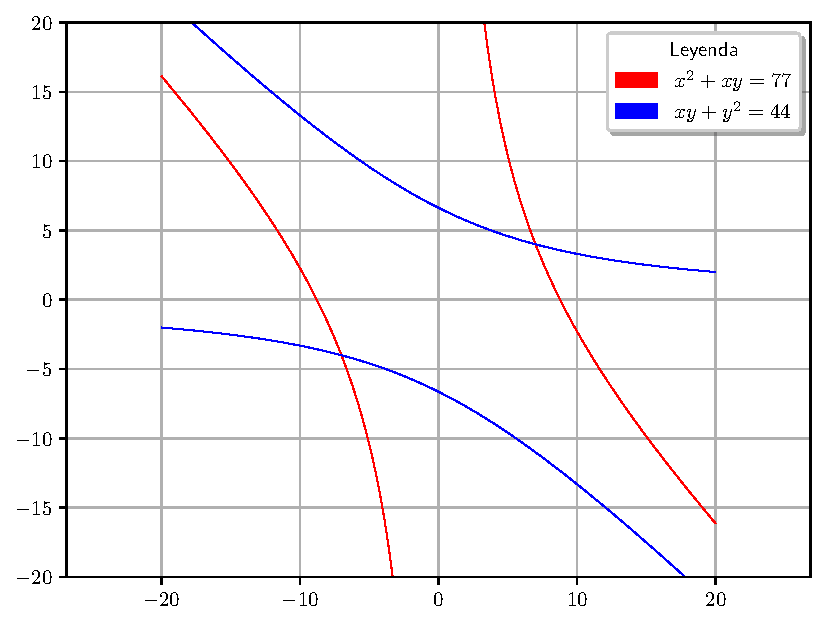
\includegraphics[width=0.45\paperwidth]{p2_plot}
		\end{figure}
	\end{solution}
\end{frame}

\begin{frame}
	\begin{solution}
		\begin{description}
			\item[Método de Newton]

				Sea
				\begin{math}
					x_{0}=
					\begin{bNiceMatrix}
						\alert{1} \\
						\alert{1}
					\end{bNiceMatrix}
				\end{math}
				un punto inicial y una tolerancia $\epsilon=10^{-5}$.
				En la etapa $k=0$, resolver el sistema lineal

				\begin{align*}
					DF
					\left(x^{\left(0\right)}\right)
					h^{\left(0\right)}             & =
					-F\left(x^{\left(0\right)}\right)              \\
					\begin{bNiceMatrix}
						2\times\alert{1}+\alert{1} & \alert{1}                  \\
						\alert{1}                  & \alert{1}+2\times\alert{1}
					\end{bNiceMatrix}
					\begin{bmatrix}
						h_{1}^{\left(0\right)} \\
						h_{2}^{\left(0\right)}
					\end{bmatrix} & =
					-\begin{bNiceMatrix}
						 \alert{1}^{2} + \alert{1}\times\alert{1} -77 \\
						 \alert{1}\times\alert{1}  + \alert{1}^{2} - 44
					 \end{bNiceMatrix} \\
					\begin{bNiceMatrix}
						3 & 1 \\
						1 & 3
					\end{bNiceMatrix}
					\begin{bmatrix}
						h_{1}^{\left(0\right)} \\
						h_{2}^{\left(0\right)}
					\end{bmatrix} & =
					-\begin{bNiceMatrix}
						 -75 \\
						 - 42
					 \end{bNiceMatrix}\xRightarrow{\text{Resolviendo}}
					\begin{bmatrix}
						h_{1}^{\left(0\right)} \\
						h_{2}^{\left(0\right)}
					\end{bmatrix}=
					\begin{bmatrix}
						\dfrac{183}{8} \\
						\dfrac{51}{8}
					\end{bmatrix}
				\end{align*}
				y actualizar
				\begin{align*}
					x^{\left(1\right)}=
					x^{\left(0\right)}+
					h^{\left(0\right)} \\
					x^{\left(1\right)}=
					\begin{bNiceMatrix}
						1 \\
						1
					\end{bNiceMatrix}+
					\begin{bNiceMatrix}
						\dfrac{183}{8} \\
						\dfrac{51}{8}
					\end{bNiceMatrix}
				\end{align*}

				% $x_{0}=\left(-1,-1\right)$.

			\item[Método de Homotopía]


		\end{description}
	\end{solution}
\end{frame}